\begin{proofbox}
\textbf{方法一：三角形两边关系（门槛最低）}

第一步：任取圆周点 $A$，连接 $OP,OA,PA$。由圆的定义，$OA=R$，已知 $OP=d$。\begin{center}
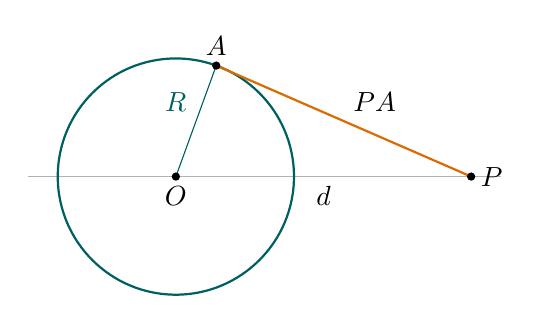
\begin{tikzpicture}[scale=.75,>=stealth]
 \coordinate (O) at (0,0); \coordinate (P) at (5,0);
 \coordinate (A) at (70:2); \coordinate (C) at (2,0); \coordinate (B) at (-2,0);
 \draw[gray!60] (-2.5,0)--(5.5,0);
 \draw[teal!75!black,thick] (O) circle (2);
 \draw[teal!75!black] (O)--(A) node[midway,above left] {$R$};
 \draw[orange!85!black,thick] (P)--(A);
 \fill (O) circle (2pt) node[below] {$O$};
 \fill (P) circle (2pt) node[right] {$P$};
 \fill (A) circle (2pt) node[above] {$A$}; \path (O)--(P) node[midway,below] {$d$}; \path (P)--(A) node[midway,above right] {$PA$};
 \end{tikzpicture}

\end{center}
第二步：由三角形两边之和不小于第三边（共线时允许等号），
\[PA\leqslant PO+OA=d+R.\]
第三步：同理 $PO\leqslant PA+AO$，两边减去 $AO$ 得
\[PA\geqslant PO-AO=d-R.\]
第四步：合并得 $d-R\leqslant PA\leqslant d+R$。

第五步：验证取等。$A=C$ 时，$P,C,O$ 依次共线，$PA=PO-CO=d-R$；$A=B$ 时，$P,O,B$ 依次共线，$PA=PO+OB=d+R$。非共线时两边均为严格不等式，因此两极值点唯一。\begin{center}
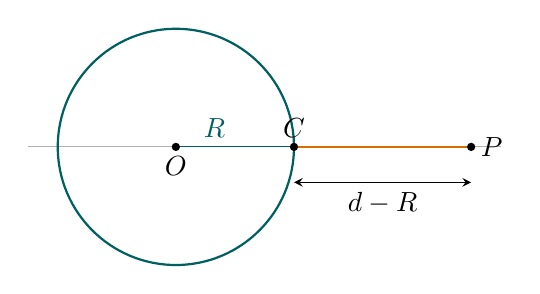
\begin{tikzpicture}[scale=.75,>=stealth]
 \coordinate (O) at (0,0); \coordinate (P) at (5,0);
 \coordinate (A) at (0:2); \coordinate (C) at (2,0); \coordinate (B) at (-2,0);
 \draw[gray!60] (-2.5,0)--(5.5,0);
 \draw[teal!75!black,thick] (O) circle (2);
 \draw[teal!75!black] (O)--(A) node[midway,above left] {$R$};
 \draw[orange!85!black,thick] (P)--(A);
 \fill (O) circle (2pt) node[below] {$O$};
 \fill (P) circle (2pt) node[right] {$P$};
 \fill (C) circle (2pt) node[above] {$C$}; \draw[<->] (2,-.6)--node[below] {$d-R$}(5,-.6);
 \end{tikzpicture}

\end{center}
\begin{center}
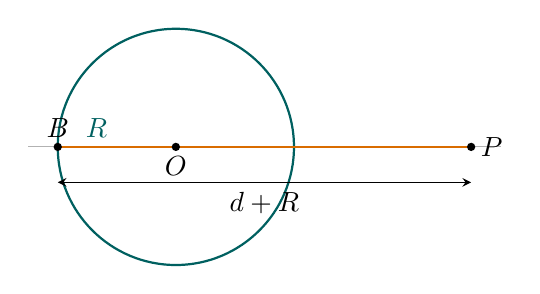
\begin{tikzpicture}[scale=.75,>=stealth]
 \coordinate (O) at (0,0); \coordinate (P) at (5,0);
 \coordinate (A) at (180:2); \coordinate (C) at (2,0); \coordinate (B) at (-2,0);
 \draw[gray!60] (-2.5,0)--(5.5,0);
 \draw[teal!75!black,thick] (O) circle (2);
 \draw[teal!75!black] (O)--(A) node[midway,above left] {$R$};
 \draw[orange!85!black,thick] (P)--(A);
 \fill (O) circle (2pt) node[below] {$O$};
 \fill (P) circle (2pt) node[right] {$P$};
 \fill (B) circle (2pt) node[above] {$B$}; \draw[<->] (-2,-.6)--node[below] {$d+R$}(5,-.6);
 \end{tikzpicture}

\end{center}

\textbf{方法二：三边关系直接夹逼（步骤最少）}

由三角形三边关系（含共线情形），
\[|OP-OA|\leqslant PA\leqslant OP+OA.\]
代入 $OP=d,OA=R,d>R$，即 $d-R\leqslant PA\leqslant d+R$。当 $A=C,B$ 时分别取等，故结论成立。此法是方法一的压缩版，并非另一独立定理。\begin{center}
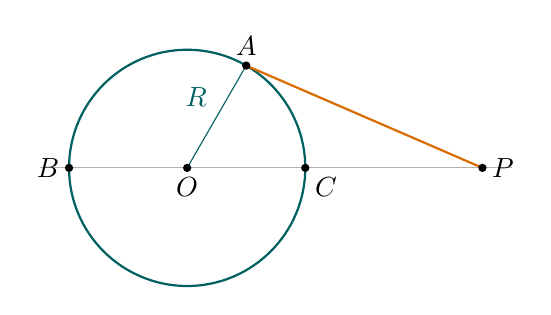
\begin{tikzpicture}[scale=.75,>=stealth]
 \coordinate (O) at (0,0); \coordinate (P) at (5,0);
 \coordinate (A) at (60:2); \coordinate (C) at (2,0); \coordinate (B) at (-2,0);
 \draw[gray!60] (-2.5,0)--(5.5,0);
 \draw[teal!75!black,thick] (O) circle (2);
 \draw[teal!75!black] (O)--(A) node[midway,above left] {$R$};
 \draw[orange!85!black,thick] (P)--(A);
 \fill (O) circle (2pt) node[below] {$O$};
 \fill (P) circle (2pt) node[right] {$P$};
 \fill (A) circle (2pt) node[above] {$A$}; \fill (C) circle (2pt) node[below right] {$C$}; \fill (B) circle (2pt) node[left] {$B$};
 \end{tikzpicture}

\end{center}

\textbf{方法三：三角换元（坐标法，便于推广）}

第一步：以 $O$ 为原点，射线 $OP$ 为 $x$ 轴正向，建立直角坐标系。则 $P=(d,0)$，圆方程为 $x^2+y^2=R^2$。

第二步：圆上任一点可表示为 $A=(R\cos\theta,R\sin\theta)$，其中 $0\leqslant\theta<2\pi$。因为 $\cos^2\theta+\sin^2\theta=1$，该表示满足圆方程，并遍历整个圆周。\begin{center}
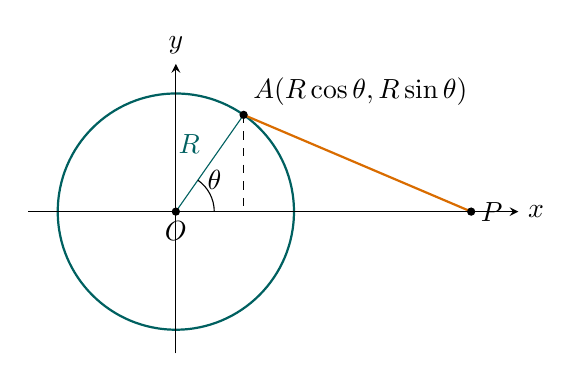
\begin{tikzpicture}[scale=.75,>=stealth]
 \coordinate (O) at (0,0); \coordinate (P) at (5,0);
 \coordinate (A) at (55:2); \coordinate (C) at (2,0); \coordinate (B) at (-2,0);
 \draw[gray!60] (-2.5,0)--(5.5,0);
 \draw[teal!75!black,thick] (O) circle (2);
 \draw[teal!75!black] (O)--(A) node[midway,above left] {$R$};
 \draw[orange!85!black,thick] (P)--(A);
 \fill (O) circle (2pt) node[below] {$O$};
 \fill (P) circle (2pt) node[right] {$P$};
 \draw[->] (-2.5,0)--(5.8,0) node[right] {$x$}; \draw[->] (0,-2.4)--(0,2.5) node[above] {$y$}; \draw[dashed] (A)--(A|-O); \draw (.65,0) arc (0:55:.65) node[right] {$\theta$}; \fill (A) circle (2pt) node[above right] {$A(R\cos\theta,R\sin\theta)$};
 \end{tikzpicture}

\end{center}
第三步：代入两点间距离公式并逐步化简：
\begin{align*}
PA^2&=(R\cos\theta-d)^2+(R\sin\theta-0)^2\\
&=R^2\cos^2\theta-2dR\cos\theta+d^2+R^2\sin^2\theta\\
&=R^2(\cos^2\theta+\sin^2\theta)+d^2-2dR\cos\theta\\
&=d^2+R^2-2dR\cos\theta.
\end{align*}
第四步：由 $-1\leqslant\cos\theta\leqslant1$，乘以负数 $-2dR$，不等号反向，整理为
\[-2dR\leqslant-2dR\cos\theta\leqslant2dR.\]
三边同时加上 $d^2+R^2$，得到
\[d^2+R^2-2dR\leqslant PA^2\leqslant d^2+R^2+2dR.\]
即 $(d-R)^2\leqslant PA^2\leqslant(d+R)^2$。

第五步：距离非负，且 $d>R$，利用平方根函数的单调性开方，得 $d-R\leqslant PA\leqslant d+R$。

第六步：$\theta=0$ 时 $\cos\theta=1$，$A=C=(R,0)$，取最小值；$\theta=\pi$ 时 $\cos\theta=-1$，$A=B=(-R,0)$，取最大值。两个角在规定范围内，故上下界均能取到。

\textbf{补充：余弦定理法（不用坐标）}
令 $\theta=\angle POA\in[0,\pi]$，非共线时余弦定理给出 $PA^2=d^2+R^2-2dR\cos\theta$；共线两端也直接满足该式。其余步骤与方法三相同。
\end{proofbox}
